\section{What a summary must remember}
\label{section:what-a-useful-summary-must-remember}

Imagine a process that moves among four states. States 1 and 2 belong to region A, and states 3 and 4 to region B. Motion within either region is fast. There are also two routes between the regions, one slow and one three times faster. A reader interested only in the probability of being in A might reasonably try to replace the four states by two.

That summary loses something immediately. Starting in state 1 or state 2 gives the same retained probability, $p_A(0)=1$, but different initial escape rates: $p_A'(0)=-1$ or $-3$ in the chosen time units. No autonomous two-state law can assign both derivatives to the same initial state. Figure~\ref{fig:dd-retention-memory} shows the missing distinction and two ways to retain its effect.
\begin{figure}[htbp]
\centering
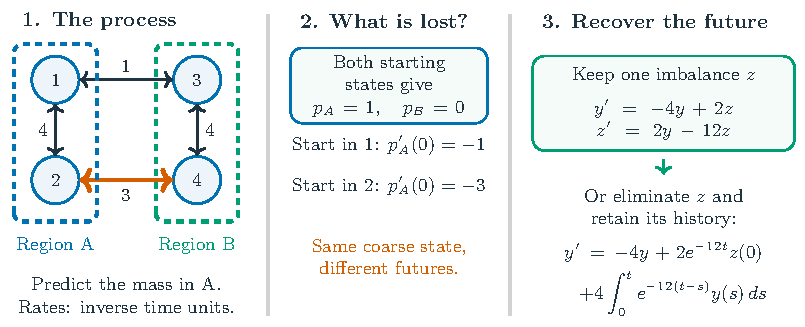
\includegraphics[width=\linewidth]{figures/portable-run-b69220b3a27348ad.result/dd-retention-memory.pdf}
\caption{What the coarse state omits. Four states exchange probability at the labelled symmetric rates. Starting in state 1 or 2 gives $p_A(0)=1$, but initial rates $-1$ and $-3$. Retaining $z=(p_1-p_2)-(p_3-p_4)$ closes the prediction for $y=p_A-p_B$, with $\dot y=-4y+2z$ and $\dot z=2y-12z$. Eliminating $z$ gives an exact memory term instead. This constructed example makes the retention and residual mechanisms explicit.}
\label{fig:dd-retention-memory}
\end{figure}

The example uses a column probability vector $p=(p_1,p_2,p_3,p_4)^T$ and the generator
\begin{equation}
 \dot p=Gp,\qquad
 G=\begin{pmatrix}
 -5&4&1&0\\
 4&-7&0&3\\
 1&0&-5&4\\
 0&3&4&-7
 \end{pmatrix},\qquad
 C=\begin{pmatrix}1&1&0&0\\0&0&1&1\end{pmatrix}.
 \label{eq:four-state}
\end{equation}
Off-diagonal entries of $G$ are transition rates and each column sums to zero, preserving total probability. The rectangular matrix $C$ retains $(p_A,p_B)^T=Cp$. It is an explicitly many-to-one map between two spaces of probability distributions.

A reconstruction map specifies what the reduced description stands for. Given a strictly positive reference distribution $\pi$, the conditional reconstruction associated with this partition is
\begin{equation}
 R=D_\pi C^T D_{C\pi}^{-1},\qquad CR=I,\qquad B=CGR,
 \label{eq:reconstruction}
\end{equation}
where $D_v$ is the diagonal matrix with vector $v$ on its diagonal. Within each coarse cell, $R$ restores the relative weights supplied by $\pi$. Here the stationary distribution is uniform, so $R=C^T/2$ and
$B=\left(\begin{smallmatrix}-2&2\\2&-2\end{smallmatrix}\right)$.
The reduced law predicts the average escape rate, not either hidden starting state separately.

The discrepancy between evolving first and reducing first is the closure residual
\begin{equation}
 \Delta=CG-BC.
 \label{eq:closure-residual}
\end{equation}
It maps a fine distribution to the difference between two proposed coarse derivatives. If $\Delta=0$, the retained state evolves autonomously for every fine initial distribution. For a partition of a Markov chain, this requires all fine states in a coarse cell to have the same total exit rate into each other coarse cell. The usual name is strong lumpability. Matching an equilibrium distribution is much weaker: with the stationary fit in Eq.~\eqref{eq:reconstruction}, $\Delta\pi=0$ even when the other states do not close.

The residual has a quantitative use beyond detecting exact failure. For finite Markov generators,
\begin{equation}
 C e^{tG}-e^{tB}C
 =\int_0^t e^{(t-s)B}\Delta e^{sG}\,ds.
 \label{eq:duhamel}
\end{equation}
Because stochastic evolution contracts the $\ell^1$ norm, a probability vector satisfies
$\|(C e^{tG}-e^{tB}C)p\|_1\leq\min\{2,t\|\Delta\|_1\}$.
Here $\|\Delta\|_1$ is the induced matrix $1$-norm. The horizon $t$ matters. A small instantaneous discrepancy may accumulate, and a bound useful for a short prediction need not justify indefinitely reusing the same reduced law.

For the four-state process, a particularly economical repair is to retain one imbalance,
\[
 y=p_1+p_2-p_3-p_4,\qquad
 z=p_1-p_2-p_3+p_4.
\]
Direct multiplication of Eq.~\eqref{eq:four-state} gives
\begin{equation}
 \dot y=-4y+2z,\qquad \dot z=2y-12z.
 \label{eq:two-coordinate}
\end{equation}
These two coordinates close exactly for the desired task, predicting $p_A=(1+y)/2$ while leaving other microstate distinctions unresolved.

Alternatively, solve the second equation for $z$ and substitute it into the first:
\begin{equation}
 \dot y(t)=-4y(t)+2e^{-12t}z(0)
       +4\int_0^t e^{-12(t-s)}y(s)\,ds.
 \label{eq:four-state-memory}
\end{equation}
The extra variable has become a memory kernel and an initial-condition term. The discarded coordinate's influence is retained through the history. Figure~\ref{fig:dd-retention-trajectories} compares the exact trajectories with the two-state approximation that omits this information.
\begin{figure}[htbp]
\centering
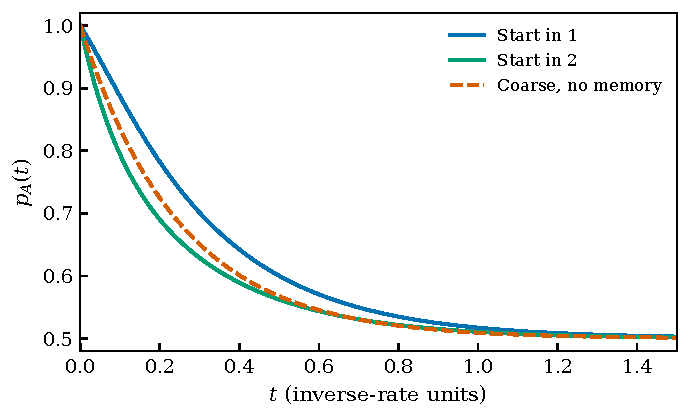
\includegraphics[width=\linewidth]{figures/portable-run-b69220b3a27348ad.result/dd-retention-trajectories.pdf}
\caption{Equal summaries, different futures. Exact region probabilities $p_A(t)$ for the four-state process, starting in state 1 or 2. The coarse model without the hidden imbalance $z$ predicts the same curve for both initial states. It initially lies between the exact trajectories but does not remain between them. Retaining $z$, or its exact memory kernel, recovers both trajectories. Time $t$ is in inverse base-rate units. The curves are analytic trajectories of Eq.~\eqref{eq:four-state}.}
\label{fig:dd-retention-trajectories}
\end{figure}

This is the elementary form of an established projection method. For a linear evolution $\dot x=Lx$, a projection $P$ and $Q=I-P$, write $u=Px$ and $w=Qx$. Exact elimination of $w$ gives
\begin{align}
 \dot u(t)={}&PLP\,u(t)+PLQ\,e^{tQLQ}w(0)\nonumber\\
 &+\int_0^t PLQ\,e^{(t-s)QLQ}QLP\,u(s)\,ds.
 \label{eq:general-memory}
\end{align}
Mori's original treatment makes clear why choosing the retained variables is decisive: a slow mode left in the discarded sector can invalidate a supposed short-memory approximation.\footnote{H. Mori, \emph{Transport, Collective Motion, and Brownian Motion}, Progress of Theoretical Physics 33 (1965),423--455, \href{https://doi.org/10.1143/ptp.33.423}{doi:10.1143/ptp.33.423}.} A local-in-time replacement needs a separation of scales or another explicit error control. Elimination alone supplies neither dissipation nor thermalisation.~\cite{Mori19656369be}

Hierarchy becomes useful when these accounts compose. If $C_{01}$ reduces level 0 to level 1 and $C_{12}$ reduces level 1 to level 2, their defects obey
\begin{equation}
 \Delta_{02}=C_{12}\Delta_{01}+\Delta_{12}C_{01}.
 \label{eq:composed-residual}
\end{equation}
The coarse model inherits the earlier mismatch as well as adding its own. A parent cannot declare itself accurate merely because it fits the already truncated child. This is the mathematical reason to transport an error account with a retained object.

Closure must still serve a task. Foundations enumerates all 2,047 bipartitions of a twelve-state model with three motifs. Its exactly closed hub/spoke partition retains essentially none of the motif-label information the task asks for. Imposing a retention requirement instead exposes a useful trade-off between predictive closure and the distinctions being preserved. The source also finds that an appropriate sign cut of the slow eigenfunction selects a good partition. The task determines which spectral or closure criterion is useful.

Each repair preserves fidelity under a specified operation. A useful summary preserves a forecast or decision. A useful reduced dynamical state carries enough information to predict its evolution. A useful hierarchy carries the inherited cost of what it discarded. These requirements give the next representation a job, rather than treating increasing abstraction as an achievement in itself.

